\section{Модели сложного теплообмена}\label{sec:$p_1$}

\subsection{Стационарная модель}\label{subsec:st}
\begin{frame}
    \frametitle{Стационарная модель}
    Область $\Omega \subset \mathbb{R}^3$, граница  $\Gamma = \partial \Omega$.
    \begin{gather}
        -a \Delta \theta + + b \kappa_a \theta^4 =  b \kappa_a \varphi,
        \quad
        - \alpha \Delta \varphi + \kappa_a \varphi = \kappa_a \theta^4,  \label{eq:pres:1}\\
        a \frac{\partial \theta}{\partial \mathbf{n}}
        +\left.\beta\left(\theta-\theta_{b}\right)\right|_{\Gamma}=0,
        \quad
        \alpha \frac{\partial \varphi}{\partial \mathbf{n}} + \gamma
        (\varphi-\theta_b^4)|_{\Gamma} = 0. \label{eq:pres:2}
    \end{gather}
    $\Omega$ -- липшицева ограниченная область, $\Gamma$ состоит из конечного числа гладких кусков,
    исходные данные удовлетворяют условиям:
    \begin{itemize}
        \item (i) $\theta_{0}, \beta, \gamma \in L^{\infty}(\Gamma),
        0 \leqslant \theta_{0} \leqslant M, \beta \geqslant \beta_{0}>0, \gamma \geqslant \gamma_{0}>0$;
    \end{itemize}
    Здесь $M, \beta_{0}, \gamma_{0}$, и $c_{0}$ положительные постоянные.
\end{frame}
%\note{
%    Стационарная нормализованная диффузионная модель, описывающая
%    радиационный, кондуктивный и конвективный теплообмен в
%    ограниченной области $\Omega \subset \mathbb{R}^3$,
%    имеет следующий вид
%    ...
%    Здесь $\theta$ -- нормализованная температура, $\varphi$ --
%    нормализованная интенсивность излучения, усредненная по всем
%    направлениям, $\textbf{v}$ -- заданное поле скоростей, $\kappa_a$ --
%    коэффициент поглощения.
%    Постоянные $a$, $b$ и $\alpha$
%    определяются следующим образом:
%    \[
%        a = \frac{k}{\rho c_v},\quad b = \frac{4\sigma n^2 T_{\max}^3}{\rho c_v},
%        \quad \alpha=\frac{1}{3\kappa - A \kappa_s},
%    \]
%    где $k$ -- теплопроводность, $c_v$ -- удельная теплоемкость, $\rho$ --
%    плотность, $\sigma$ -- постоянная Стефана-Больцмана, $n$ --
%    показатель преломления, $T_{\max}$ -- максимальная температура в
%    ненормализованной модели, $\kappa = \kappa_s + \kappa_a$ -- коэффициент
%    полного взаимодействия, $\kappa_s$ -- коэффициент рассеяния.
%    Коэффициент $A \in [-1, 1]$ описывает анизотропию рассеяния, случай
%    $A=0$ соответствует изотропному рассеянию.
%
%    Будем предполагать, что функции $\theta$ и $\varphi$, описывающие
%    процесс сложного теплообмена, удовлетворяют следующим условиям на
%    границе $\Gamma = \partial \Omega$: ...
%}


\begin{frame}
    \begin{definition}
        Пара
        $\{\theta, \varphi\} \in H^1(\Omega) \times H^1(\Omega)$ называется слабым решением задачи,
        если для любых $\eta, \psi \in H^1(\Omega)$ выполняются равенства:
        \begin{gather*}
            a(\nabla \theta, \nabla \eta)
            + \left(b \kappa_{a}\left(|\theta| \theta^{3} - \varphi\right), \eta\right)
            + \int_{\Gamma} \beta\left(\theta - \theta_{0}\right) \eta d \Gamma=0, \\
            \alpha(\nabla \varphi, \nabla \psi)+\kappa_{a}\left(\varphi-|\theta| \theta^{3},
            \psi\right)+\int_{\Gamma} \gamma\left(\varphi-\theta_{0}^{4}\right) \psi d \Gamma=0.
        \end{gather*}
    \end{definition}
    \begin{theorem}[Chebotarev, 2015]
        Пусть выполняются условия (i).
        Тогда существует единственное слабое
        решение задачи~\eqref{eq:pres:1}--\eqref{eq:pres:2},
        удовлетворяющее неравенствам:
        \begin{align}
            & a\|\nabla \theta\|^{2} \leqslant b \kappa_{a} M^{5}|\Omega|
            + \|\gamma\|_{L^{\infty}(\Gamma)} M^{2}|\Gamma|,\\
            & \alpha\|\nabla \varphi\|^{2} \leqslant \kappa_{a} M^{8}|\Omega|
            + \|\beta\|_{L^{\infty}(\Gamma)} M^{8}|\Gamma|,\\
            & 0 \leqslant \theta \leqslant M, \quad 0 \leqslant \varphi \leqslant M^{4}.
        \end{align}
    \end{theorem}
\end{frame}

\subsection{Квазистационарная модель}\label{subsec:qst}
\begin{frame}
    \frametitle{Квазистационарная модель}
    \begin{align}
        \frac{\partial\theta}{\partial t} - a\Delta\theta
        + b\kappa_a (|\theta|\theta^3 - \phi) &= 0, \label{eq:1_5:1}\\
        - \alpha\Delta\phi + \kappa_a (\phi - |\theta|\theta^3 ) &= 0,
        \quad x \in \Omega, \quad 0 < t < T ; \label{eq:1_5:1+} \\
        a \frac{\partial \theta}{\partial n}
        +\left.\beta\left(\theta-\theta_{b}\right)\right|_{\Gamma}&=0,
        \quad \alpha \frac{\partial \varphi}{\partial \mathbf{n}} + \gamma
        (\varphi-\theta_b^4)|_{\Gamma} = 0 \text{ на } \Gamma; \label{eq:1_5:2} \\
        \theta|_{t=0} &= \theta_0. \label{eq:1_5:3}
    \end{align}
    Предполагаем, что
    \begin {itemize}
        \item (j) $a, b, \alpha, \kappa_{a} =$ Const $>0$,
        \item (jj) $\theta_{b}, q_{b}, u=\theta^4_b \in U, r
        =a\left(\theta_{b}+q_{b}\right) \in L^{5}(\Sigma), \; \theta_{0} \in L^{5}(\Omega)$.
    \end{itemize}

    Здесь $\Sigma = \Gamma \times (0, T)$, $U$ -- пространство $L^{2}(\Sigma)$ с нормой
    \[
        \|u\|_{\Sigma}=\left(\int_{\Sigma} u^{2} d \Gamma d t\right)^{1/2}.
    \]
\end{frame}


\begin{frame}
    Определим операторы $A: V \rightarrow V^{\prime}, B: U \rightarrow V^{\prime}$,
    которые выполняются для любых $y, z \in V, w \in L^{2}(\Gamma)$:
    \[
        (A y, z)=(\nabla y, \nabla z)+\int_{\Gamma} y z d \Gamma, \quad(B w, z)=\int_{\Gamma} w z d \Gamma.
    \]

    \begin{definition}
        Пара $\theta \in W, \varphi \in L^{2}(0, T ; V)$
        называется слабым решением задачи~\eqref{eq:1_5:1}--\eqref{eq:1_5:3}
        если
        \begin{equation*}
            \theta^{\prime}+a A \theta+b \kappa_{a}\left([\theta]^{4}-\varphi\right)=B r,
            \quad \theta(0)=\theta_{0}, \quad \alpha A \varphi+\kappa_{a}\left(\varphi-[\theta]^{4}\right)=B u.
        \end{equation*}
    \end{definition}
    Здесь и далее будем обозначать через
    $[\theta]^s \coloneqq |\theta|^s \mathrm{sign}\theta,\quad s \in \mathbb{R}$.
    \begin{lemma}[1.20]
        Пусть выполняются условия (j), (jj).
        Тогда существует единственное слабое решение задачи~\eqref{eq:1_5:1}--\eqref{eq:1_5:3} и справедливо
        \[
            \psi=[\theta]^{5 / 2} \in L^{\infty}(0, T ; H) \cap L^{2}(0, T ; V),
            \quad[\theta]^{4} \in L^{2}(0, T ; H).
        \]
    \end{lemma}
\end{frame}

\subsection{Квазилинейная модель}\label{subsec:ql}
\begin{frame}
    \frametitle{Квазилинейная модель}
    \begin{gather}
        \sigma \partial \theta / \partial t
        -\operatorname{div}(k(\theta) \nabla \theta)
        +b\left(\theta^{3}|\theta|-\varphi\right)=f, \label{eq:1_6:1}\\
        -\operatorname{div}(\alpha \nabla \varphi)
        +\beta\left(\varphi-\theta^{3}|\theta|\right)=g, x \in \Omega, 0<t<T, \label{eq:1_6:2}\\
        k(\theta) \partial_{n} \theta+\left.p\left(\theta-\theta_{b}\right)\right|_{\Gamma}=0,
        \alpha \partial_{n} \varphi
        +\left.\gamma\left(\varphi-\theta_{b}^{4}\right)\right|_{\Gamma}=0,
        \left.\quad \theta\right|_{t=0}=\theta_{in}.\label{eq:1_6:3}
    \end{gather}

    Предполагаем, что:
    \begin{itemize}
        \item (k1) $\alpha, \beta, \sigma \in L^{\infty}(\Omega),
        \quad b=r \beta, r = Const > 0; \alpha \geq \alpha_{0}, \beta \geq \beta_{0},
        \sigma \geq \sigma_{0}, \alpha_{0}, \beta_{0}, \sigma_{0}=$ Const $>0$.

        \item (k2) $0<k_{0} \leq k(s) \leq k_{1},\left|k^{\prime}(s)\right| \leq k_{2},
        s \in \mathbb{R}, \quad k_{j}=$ Const.

        \item (k3) $0 \leq \theta_{b} \in L^{\infty}(\Sigma), 0 \leq \theta_{\text{in}}
        \in L^{\infty}(\Omega)$; $\gamma_{0} \leq \gamma \in L^{\infty}(\Gamma), p_{0}
        \leq p \in L^{\infty}(\Gamma), \gamma_{0}, p_{0}=$ Const $>0$.

        \item (k4) $0 \leq f, g \in L^{\infty}(Q).$
    \end{itemize}

\end{frame}


\begin{frame}
    Определим операторы $A_{1}: V \rightarrow V_{0}^{\prime}$ и $A_{2}: V \rightarrow V^{\prime}$
    такие, что для всех $\theta, \varphi, v \in V$ выполняются следующие равенства:
    \[
        \begin{gathered}
            \left(A_{1}(\theta), v\right)=(k(\theta) \nabla \theta, \nabla v)
            +\int_{\Gamma} p \theta v d \Gamma=(\nabla h(\theta), \nabla v)
            +\int_{\Gamma} p \theta v d \Gamma, \\
            \left(A_{2} \varphi, v\right)=(\alpha \nabla \varphi, \nabla v)
            +\int_{\Gamma} \gamma \varphi v d \Gamma,
        \end{gathered}
    \]
    где $ h(s)=\int_{0}^{s} k(r) d r$.


    \begin{definition}
        Пару $\theta \in W, \varphi \in L^{2}(0, T ; V)$ будем называть слабым
        решением задачи~\eqref{eq:1_6:1}--\eqref{eq:1_6:3}, если
        \begin{equation}
            \label{eq:1_6:4}
            \sigma \theta^{\prime}+A_{1}(\theta)+b\left([\theta]^{4}-\varphi\right)=f_{b}+f
            \quad \text { п. в. в }(0, T), \quad \theta(0)=\theta_{\text{in}},
        \end{equation}
        \begin{equation}
            \label{eq:1_6:5}
            A_{2} \varphi+\beta\left(\varphi-[\theta]^{4}\right)
            =g_{b}+g \quad \text { п. в. в }(0, T).
        \end{equation}
    \end{definition}
    Здесь $f_{b}, g_{b} \in L^{2}\left(0, T ; V^{\prime}\right)$ и
    \[
        \left(f_{b}, v\right)=\int_{\Gamma} p \theta_{b} v d \Gamma,
        \quad\left(g_{b}, v\right)=
        \int_{\Gamma} \gamma \theta_{b}^{4} v d \Gamma \quad \forall v \in V.
    \]
\end{frame}

\begin{frame}
    Рекурсивно определим последовательность
    $\theta_{m} \in W, \quad \varphi_{m} \in L^{2}(0, T ; V)$ такую, что
    \begin{equation}
        \label{eq:1_6:10}
        \theta_{m}=F_{2}\left(\theta_{m-1}, \varphi_{m-1}\right),
        \quad \varphi_{m}=F_{1}\left(\theta_{m}\right), \quad m=1,2, \ldots
    \end{equation}
    Здесь операторы $F_{1}: L^{\infty}(\Omega) \rightarrow V$ и
    $F_{2}: L^{\infty}(Q) \times L^{2}(0, T ; V) \rightarrow W$ определены следующим образом.
    Пусть $\varphi=F_{1}(\theta)$, если
    \begin{equation}
        \label{eq:1_6:6}
        A_{2} \varphi+\beta\left(\varphi-[\theta]^{4}\right)=g_{b}+g,
    \end{equation}
    и $\theta=F_{2}(\zeta, \varphi)$, если
    \begin{equation}
        \label{eq:1_6:7}
        \sigma \theta^{\prime}+A(\zeta, \theta)
        +b\left([\theta]^{4}-\varphi\right)=f_{b}+f
        \quad \text { п. в. в }(0, T), \quad \theta(0)=\theta_{i n}.
    \end{equation}
    Здесь
    $ (A(\zeta, \theta), v)=(k(\zeta) \nabla \theta, \nabla v) +\int_{\Gamma} p \theta v d \Gamma \quad \forall v \in V$,
    \[
        W=\left\{y \in L^{2}(0, T ; V): \sigma y^{\prime}=\sigma d y / d t \in L^{2}
        \left(0, T, V^{\prime}\right)\right\}.
    \]

\end{frame}

\begin{frame}
    \frametitle{Существование решения квазилинейной задачи}
    \begin{lemma}
        \label{lm:1_6:3}
        Если выполнены условия (k1)--(k4), то существует константа $C>0$,
        не зависящая от $m$, такая, что
        \begin{gather*}
            \left\|\varphi_{m}\right\|_{L^{2}(0, T ; V)} \leq C,
            \quad\left\|\theta_{m}\right\|_{L^{2}(0, T ; V)} \leq C, \\
            \int_{0}^{T-\delta}\left\|\theta_{m}(s+\delta)
            -\theta_{m}(s)\right\|^{2} d s \leq C \delta.
        \end{gather*}
    \end{lemma}

    \begin{equation*}
        \begin{aligned}
            & \theta_{m} \rightarrow \widehat{\theta} \text { слабо в } L^{2}(0, T ; V),
            \text { сильно в } L^{2}(0, T ; H), \\
            & \varphi_{m} \rightarrow \widehat{\varphi} \text { слабо в } L^{2}(0, T ; V).
        \end{aligned}
    \end{equation*}

    \begin{theorem}
        \label{th:1_6:1}
        Если выполнены условия (k1)--(k4), то существует хотя бы одно
        решение задачи~\eqref{eq:1_6:1}--\eqref{eq:1_6:3}.
    \end{theorem}

\end{frame}

\begin{frame}
    \frametitle{Теорема единственности и сходимость итеративного метода}
    \begin{theorem}
        Если выполнены условия (k1)--(k4) и $\theta_{*}, \varphi_{*}$ является
        решением задачи~\eqref{eq:1_6:1}--\eqref{eq:1_6:3}
        так, что $\theta_{*}, \nabla \theta_{*} \in L^{\infty}(Q)$,
        то других ограниченных решений этой задачи нет.
    \end{theorem}


    \begin{theorem}
        Если выполнены условия (k1)--(k4) и $\theta_{*}, \varphi_{*}$ является
        решением задачи~\eqref{eq:1_6:1}--\eqref{eq:1_6:3}
        так, что $\theta_{*}, \nabla \theta_{*} \in L^{\infty}(Q)$.
        Тогда для последовательностей~\eqref{eq:1_6:10} справедливы следующие сходимости:
        \[
            \theta_{m} \rightarrow \theta_{*} \quad \text { в } L^{2}(0, T ; V),
            \quad \varphi_{m} \rightarrow \varphi_{*} \quad \text { в } L^{2}(0, T ; V).
        \]
    \end{theorem}

\end{frame}


\section{Граничные обратные задачи и задачи с данными Коши}\label{sec:rev}

\subsection{Граничная обратная задача}\label{subsec:rev}
\begin{frame}
    \frametitle{Граничная обратная задача}
    Модель имеет следующий вид
    \begin{equation}
        \label{eq:2_1:initial}
        - a \Delta \theta + b \kappa_a(\theta ^ 3 | \theta | - \varphi) = 0,  \quad
        - \alpha \Delta \varphi + \kappa_a (\varphi - \theta ^3 | \theta |) = 0,
    \end{equation}
    и дополняется граничными условиями на
    $\Gamma \coloneqq \partial \Omega =\overline{\Gamma}_0 \cup \overline{\Gamma}_1 \cup \overline{\Gamma}_2$,
    где части границы $\Gamma_0, \Gamma_1, \Gamma_2$ не имеют пересечений:

    \begin{equation}
        \label{eq:2_1:initial-boundary}
        \begin{aligned}
            \Gamma &: \; a \partial_n \theta + \beta (\theta - \theta _b) = 0, \\
            \Gamma_0 \cup \Gamma_2 &: \; \alpha \partial_n \varphi
            + \gamma(\varphi - \theta_b ^4 ) = 0, \\
            \Gamma_1 &: \; \alpha \partial_n \varphi + u(\varphi - \theta_b ^4 ) = 0. \\
        \end{aligned}
    \end{equation}

    Функции $\gamma, \theta_b, \beta$ известны.
    Неизвестная функция $u$ характеризует отражающие свойства участка границы $\Gamma_1$.
    Предполагается, что $0 < u_1 \leq u \leq u_2$.

    \textbf{Обратная задача} заключается в отыскании тройки $\theta, \varphi, u$
    по дополнительному условию $\theta|_{\Gamma_2} = \theta_0$.

    \textbf{Экстремальная задача} заключается в минимизации функционала
    \[ J(\theta) = \frac{1}{2} \int_{\Gamma_2} (\theta - \theta_0)^2 d\Gamma. \]
\end{frame}


\begin{frame}
    \frametitle{Существование решения и условия оптимальности}
    Будем предполагать что исходные данные удовлетворяют условию
    \begin{itemize}
        \item $\text{(i)}\;\beta\in L^\infty(\Gamma); \gamma \in L^\infty(\Gamma_0\cup\Gamma_2);$
        $u_1, u_2 \in L^\infty(\Gamma_1);$
        $0 < \beta_0 \le \beta; 0 < \gamma_0 \le \gamma;\; \beta_0,\gamma_0=Const,$
        $0 \le u_1 \le u_2$.
    \end{itemize}
    \begin{theorem}
        Пусть выполняется условие (i).
        Тогда существует хотя бы одно решение задачи оптимального управления.
    \end{theorem}

    \begin{theorem}
        \label{th:2_1:2}
        Пусть $\hat{y}=\{\hat{\theta},\hat{\varphi} \} \in Y, \hat{u} \in U_{ad}$
        --- решение экстремальной задачи.
        Тогда существует пара $p = (p_1, p_2)$, $p \in Y$
        такая, что тройка $(\hat{y}, \hat{u}, p)$, удовлетворяет следующим условиям:
        \begin{gather*}
            A_1 p_1 + 4 |\hat{\theta}|^3 \kappa_a(b p_1 - p_2) = f_c,
            \;\; (f_c,v) = - \int_{\Gamma_2} (\hat{\theta} - \theta_0) v d\Gamma, \\
            A_2 p_2 + \kappa_a (p_2-b p_1) = g_c(p_2, \hat{u}),
            \;(g_c(p_2, \hat{u}), v) = -\int_{\Gamma_1} \hat{u} p_2 v d\Gamma, \\
            \int_{\Gamma_1} p_2 (\hat{\varphi} - \theta_b^4)(u-w) d\Gamma
            \leq 0 \quad \forall w \in U_{ad}.
        \end{gather*}
    \end{theorem}
\end{frame}

\subsection{Обратная задача с условиями типа Коши}\label{subsec:rev_koshi}
\begin{frame}
    \frametitle{Задача без краевых условий для интенсивности излучения}
    \begin{equation}
        \label{eq:2_2:eq1}
        - a \Delta \theta + b \kappa_a(\theta ^ 3 | \theta | - \varphi) = 0,  \quad
        - \alpha \Delta \varphi + \kappa_a (\varphi - \theta ^3 | \theta |) = 0,
    \end{equation}
    На $\Gamma$ известно температурное поле и тепловой поток:
    \begin{equation}
        \label{eq:2_2:bc2} \theta = \theta_b, \quad \partial_n\theta = q_b.
    \end{equation}
    Заменяем на <<искусственные>> краевые условия
    \begin{equation}
        \label{eq:2_2:bc3}
        a(\partial_n\theta+\theta) = r,\;\;
        \alpha(\partial_n\varphi+\varphi) = u \text{ на }\Gamma.
    \end{equation}
    Функция $r(x),\, x\in\Gamma$ является заданной, а неизвестная функция $u(x),\, x\in\Gamma$
    играет роль управления.

    \textbf{Экстремальная задача} заключается в отыскании тройки
    $\{\theta_\lambda,\varphi_\lambda,u_\lambda\}$ такой, что
    \begin{equation}
        \label{eq:2_2:cost}
        J_\lambda(\theta, u) = \frac{1}{2}\int\limits_\Gamma (\theta - \theta_b)^2 d\Gamma
        + \frac{\lambda}{2}\int\limits_\Gamma u^2 d\Gamma \rightarrow\inf
    \end{equation}
    на решениях краевой задачи.
\end{frame}

\begin{frame}
    Будем предполагать, что
    \begin{itemize}
        \item $(j) \;\; a,b,\alpha,\kappa_a, \lambda ={\textrm Const}> 0,$
        \item $(jj) \;\, \theta_b, \,q_b \in U,\;\; r=a(\theta_b+q_b)$.
    \end{itemize}
    Определим оператор ограничений $F(\theta, \varphi, u) : V \times V \times U \rightarrow V' \times V'$,
    \[
        F(\theta, \varphi, u) = \{ aA\theta + b \kappa_a ( [\theta]^4- \varphi) - Br,\;
        \alpha A \varphi + \kappa_a (\varphi -[\theta]^4) - Bu\}.
    \]


    \textbf{Задача $CP$.} Найти тройку $\{\theta, \varphi, u \} \in V \times V \times U$ такую, что
    \begin{equation}
        \label{eq:2_2:cp}
        J_\lambda(\theta, u) \equiv \frac{1}{2}\|\theta -\theta_b\|^2_\Gamma
        + \frac{\lambda}{2}\|u\|^2_\Gamma \rightarrow \inf,\;\; F(\theta, \varphi, u)=0.
    \end{equation}
\end{frame}

\begin{frame}
    \frametitle{Разрешимость задачи $CP$ и условия оптимальности}

    \begin{theorem}
        \label{th:2_2:1}
        Пусть выполняются условия $(j), (jj)$.
        Тогда существует решение задачи $CP$.
    \end{theorem}
    \begin{theorem}
        \label{th:2_2:2}
        Пусть выполняются условия (j),(jj).
        Если $\{\hat{\theta}, \hat{\varphi}, \hat{u}\}$ -- решение задачи $CP$,
        то существует единственная пара $\{p_1, p_2 \} \in V\times V$ такая, что
        \begin{equation}
            \label{eq:2_2:as}
            aAp_1 +4|\hat{\theta}|^3 \kappa_a(bp_1 - p_2) = B(\theta_b - \hat{\theta}), \;\;
            \alpha A p_2 + \kappa_a (p_2 - b p_1)=0
        \end{equation}
        и при этом $\lambda\hat{u} = p_2$.
    \end{theorem}
\end{frame}


\begin{frame}
    \frametitle{Аппроксимация задачи с условиями типа Коши}
    \begin{theorem}
        \label{th:2_2:3}
        Пусть выполняются условия (j),(jj) и существует решение
        задачи~\eqref{eq:2_2:eq1}--\eqref{eq:2_2:bc2}.
        Если $\{\theta_\lambda,\varphi_\lambda,u_\lambda\}$ -- решение
        задачи $CP$ для $\lambda>0$, то существует последовательность $\lambda\to +0$
        такая, что
        \[
            \theta_\lambda\rightarrow\theta_*, \;\; \varphi_\lambda\rightarrow\varphi_*
            \text{ слабо в }V,\text{ сильно в }H,
        \]
        где $\theta_*,\varphi_*$ -- решение задачи~\eqref{eq:2_2:eq1}--\eqref{eq:2_2:bc2}.
    \end{theorem}


    Из ограниченности последовательности $u_\lambda$
    в пространстве $U$ следует
    ее слабая относительная компактность и существование последовательности
    (возможно не единственной) $\lambda\to+0$ такой, что
    $u_\lambda \rightarrow u_*$ слабо в $U$.

%    Для практического решения задачи~\eqref{eq:2_2:eq1}--\eqref{eq:2_2:bc2} важно то,
%    что \textit{для любой последовательности} $\lambda\to+0$ справедлива оценка
%    $\|\theta_\lambda -\theta_b\|^2_\Gamma\leq C\lambda$,
%    а поскольку $\partial_n\theta_\lambda=\theta_b+q_b-\theta_\lambda$,
%    то также $\|\partial_n\theta_\lambda-q_b\|^2_\Gamma\leq C\lambda$.
%    Указанные неравенства гарантируют, что граничные значения
%    $\theta_\lambda,\,\partial_n\theta_\lambda$ при малых $\lambda$
%    аппроксимируют краевые условия задачи~\eqref{eq:2_2:eq1}--\eqref{eq:2_2:bc2}.
\end{frame}

\subsection{Квазистационарная задача с данными Коши}\label{subsec:qst_koshi}
\begin{frame}
    \frametitle{Квазистационарная модель с данными Коши}
    \begin{equation}
        \label{eq:2_3:1}
        \begin{split}
            & \frac{\partial \theta}{\partial t} - a \Delta \theta
            + b \kappa_{a} \left(|\theta| \theta^{3}-\varphi\right) = 0,\\
            & - \alpha \Delta \varphi
            + \kappa_{a} \left(\varphi-|\theta| \theta^{3}\right) = 0,
            \quad x \in \Omega, \quad 0 < t < T;
        \end{split}
    \end{equation}
    \begin{align}
        a \left(\partial_{n} \theta+\theta\right)=r,
        & \quad \alpha\left(\partial_{n} \varphi
        + \varphi\right) = u \text { на } \Gamma;  \label{eq:2_3:2}\\
        & \left.\theta\right|_{t=0} = \theta_{0}. \label{eq:2_3:3}
    \end{align}


    \textbf{Экстремальная задача} состоит в том, чтобы найти тройку
    $\left\{\theta_{\lambda}, \varphi_{\lambda}, u_{\lambda}\right\}$ такую, что
    \begin{equation}
        \label{eq:2_3:4}
        J_{\lambda}(\theta, u)=\frac{1}{2} \int_{0}^{T}
        \int_{\Gamma}\left(\theta-\theta_{b}\right)^{2} d \Gamma d t+\frac{\lambda}{2}
        \int_{0}^{T} \int_{\Gamma} u^{2} d \Gamma d t \rightarrow \inf
    \end{equation}
    на решениях задачи~\eqref{eq:2_3:1}--\eqref{eq:2_3:3}.
\end{frame}

\begin{frame}
    \frametitle{Задача оптимального управления $OC$}
    Будем считать, что
    \begin{itemize}
        \item $(k)\; a, b, \alpha, \kappa_{a}, \lambda=$ Const $>0$,
        \item $(kk)\; \theta_{b}, q_{b} \in U, r=a\left(\theta_{b}+q_{b}\right)
        \in L^{5}(\Sigma), \; \theta_{0} \in L^{5}(\Omega)$.
    \end{itemize}

    Задача оптимального управления $OC$ заключается в отыскании тройки
    $\{\theta, \varphi, u\} \in W \times L^{2}(0, T ; V) \times U$ такой, что
    \[
        J_{\lambda}(\theta, u) \equiv \frac{1}{2}\left\|\theta-
        \theta_{b}\right\|_{\Sigma}^{2}+
        \frac{\lambda}{2}\|u\|_{\Sigma}^{2}
        \rightarrow \inf, \quad F(\theta, \varphi, u)=0.
    \]
    Здесь и далее
    $
    W=\left\{y \in L^{2}(0, T ; V):y^{\prime}
    \in L^{2}\left(0, T, V^{\prime}\right)\right\}
    $.

    \begin{theorem}
        \label{th:2_3:1}
        Пусть выполняются условия $(k), (kk)$.
        Тогда существует решение задачи $OC$.
    \end{theorem}
    Определим операторы $A: V \rightarrow V^{\prime}, B: U \rightarrow V^{\prime}$
    \[
        (A y, z)=(\nabla y, \nabla z)+\int_{\Gamma} y z d \Gamma,
        \quad(B w, z)=\int_{\Gamma} w z d \Gamma,\quad y, z \in V, w \in L^{1}(\Gamma).
    \]

\end{frame}

\begin{frame}
    \frametitle{Условия оптимальности и аппроксимация обратной задачи}


    \begin{theorem}
        \label{th:2_3:2}
        Пусть выполнены условия $(k), (kk)$.
        Если $\{\widehat{\theta}, \widehat{\varphi}, \widehat{u}\}$ — решение задачи $OC$,
        то существует единственная пара $\left\{p_ {1}, p_{2}\right\} \in W \times W$ такая, что
        \begin{equation}
            \label{eq:2_3:15}
            \begin{aligned}
                -p_{1}^{\prime}+a A p_{1}+4|\widehat{\theta}|^{3} \kappa_{a}\left(b p_{1}
                -p_{2}\right)&=B\left(\theta_{b}-\widehat{\theta}\right), \;
                p_{1}(T)=0, \\
                \alpha A p_{2}+\kappa_{a}\left(p_{2}-b p_{1}\right)&=0,
                \quad \lambda \widehat{u}=\left.p_{2}\right|_{\Sigma}.
            \end{aligned}
        \end{equation}
    \end{theorem}

    \begin{theorem}
        \label{th:2_3:3}
        Пусть выполняются условия $(k), (kk)$ и существует решение
        $\theta, \varphi \in$ $L^{2}\left(0, T ; H^{2}(\Omega) \right)$
        задачи~\eqref{eq:2_3:1}--\eqref{eq:2_3:3}.
        Если $\left\{\theta_{\lambda}, \varphi_{\lambda}, u_{\lambda}\right\}$
        — решение задачи $OC$ при $\lambda>0$, то при $\lambda\rightarrow+0$
        \[
            \begin{gathered}
                \theta_{\lambda} \rightarrow \theta \text { слабо в } L^{2}(0, T ; V),
                \text { сильно в } L^{2}(Q), \\
                \varphi_{\lambda} \rightarrow \varphi \text { слабо в } L^{2}(0, T ; V).
            \end{gathered}
        \]
    \end{theorem}
\end{frame}

\subsection{Стационарная задача с условиями Коши для температуры на части границы}\label{subsec:st-koshi}
\begin{frame}
    \frametitle{Стационарная задача с условиями Коши для температуры на части границы}
    Область $\Omega\subset \mathbb{R}^3$ с границей $\Gamma=\partial\Omega$.
    \begin{equation}
        \label{eq:2_4:eq1}
        - a\Delta\theta + b\kappa_a(|\theta|\theta^3- \varphi)=0,   \quad
        -\alpha \Delta \varphi + \kappa_a(\varphi-|\theta|\theta^3)=0,\; x\in\Omega.
    \end{equation}
    $\Gamma \coloneqq \partial \Omega =\overline{\Gamma}_1 \cup \overline{\Gamma}_2$
    так, что $\Gamma_1 \cap \Gamma_2 =  \emptyset$.
    На всей границе $\Gamma$ задается тепловой поток $q_b$,
    \begin{equation}
        \label{eq:2_4:bc1}
        a\partial_n\theta = q_b, \quad x\in \Gamma.
    \end{equation}
    Для задания краевого условия для интенсивности излучения требуется знать функцию $\gamma$.
    В случае, если эта функция неизвестна на части границы $\Gamma_2$,
    краевое условие для интенсивности излучения на $\Gamma_2$ не ставится, а в качестве условия
    переопределения на $\Gamma_1$, в дополнение к условию на
    $\varphi$, задается температурное поле $\theta_b$,
    \begin{equation}
        \label{eq:2_4:bc2}
        \alpha\partial_n\varphi + \gamma (\varphi - \theta_b ^4 ) = 0,\;
        \theta=\theta_b\quad \text{ на } \Gamma_1.
    \end{equation}.


\end{frame}

\begin{frame}
    \frametitle{Постановка задачи управления}
    Введем новую неизвестную функцию
    $\psi= a\theta + \alpha b \varphi$.

    \textbf{Краевая задача}:
    \begin{equation}
        \label{eq:2_4:eq2}
        - a \Delta \theta + g (\theta) = \frac{\kappa_a}{\alpha}\psi, \quad
        \Delta \psi = 0, \; x \in \Omega,
    \end{equation}
    \begin{equation}
        \label{eq:2_4:bc3}
        a \partial_n \theta = q_b \; \text{ на }\Gamma, \;\;
        \alpha \partial_n \psi + \gamma \psi  =  r,\;\;
        \theta = \theta_b  \text{ на }\Gamma_1.
    \end{equation}
    Здесь $g(\theta) = b \kappa_a|\theta|\theta^3 + \frac{a\kappa_a}{\alpha}\theta$, $r=\alpha b \gamma \theta_b^4+ \alpha q_b + a \gamma \theta_b$.


    Задача \textbf{оптимального управления}, аппроксимирующая краевую задачу,
    заключается в отыскании тройки $\{\theta_\lambda,\psi_\lambda,u_\lambda\}$ такой, что
    \begin{gather}
        \label{eq:2_4:cost}
        J_\lambda(\theta, u) =
        \frac{1}{2} \int \limits_{\Gamma_1} (\theta - \theta_b)^2 d \Gamma
        + \frac{\lambda}{2}\int\limits_{\Gamma_2} u^2 d\Gamma \rightarrow \inf, \\
        - a \Delta \theta + g (\theta) = \frac{\kappa}{\alpha}\psi, \quad
        \Delta \psi = 0, \; x \in \Omega, \\
        a \partial_n \theta + s \theta = q_b + s \theta_b,
        \; \alpha \partial_n \psi + \gamma \psi = r
        \text{ на } \Gamma_1,\\
        a \partial_n \theta = q_b, \;
        \alpha \partial_n \psi = u \text{ на } \Gamma_2.
    \end{gather}
    $\lambda, s > 0$ -- регуляризирующие параметры.

\end{frame}

% на слайде отсутсвуют определения f_1 и f_2
\begin{frame}
    \frametitle{Разрешимость задачи оптимального управления}
    Будем предполагать, что исходные данные удовлетворяют условиям:
    \begin{itemize}
        \item $(l) \; a,b,\alpha,\kappa_a, \lambda, s ={\textrm Const}> 0.$
        \item $(ll) \; 0<\gamma_0\leq \gamma \in L^\infty(\Gamma_1), \; \theta_b, r \in L^2(\Gamma_1),\; q_b\in L^2(\Gamma)$.
    \end{itemize}
    \textbf{Задача $(P_\lambda)$.} Найти тройку
    $\{\theta_\lambda, \psi_\lambda, u_\lambda \} \in V \times V \times U$
    такую, что
    \begin{equation}
        \label{eq:2_4:cp}
        J_\lambda(\theta, u) = \frac{1}{2}\|\theta -\theta_b\|^2_{L^2(\Gamma_1)}
        + \frac{\lambda}{2}\|u\|^2_U \rightarrow \inf,\;\; F(\theta, \psi, u) = 0.
    \end{equation}
    Здесь $F(\theta, \psi, u) : V \times V \times U \rightarrow V' \times V'$,
    \begin{gather*}
    (A_1 y,z)
        =a (\nabla y, \nabla z) +
        s\int\limits_{\Gamma_1}yz d\Gamma, \;\;
        (A_2 y,z) =\alpha (\nabla y, \nabla z)
        + \int\limits_{\Gamma_1}\gamma yz d\Gamma, \\
        (B_1 f, v) = \int\limits_{\Gamma_1}fv d\Gamma,\;\;
        (B_2 h, w) = \int\limits_{\Gamma_2}hw d\Gamma.
    \end{gather*}
    \[
        F(\theta, \psi, u) = \left\{A_1\theta + g(\theta) - \frac{\kappa_a}{\alpha}\psi - f_1,\; A_2 \psi - f_2 - B_2 u \right\}.
    \]

    \begin{theorem}
        \label{th:2_4:1}
        При выполнении условий $(l), (ll)$ существует решение задачи $(P_\lambda)$.
    \end{theorem}
\end{frame}

\begin{frame}
    \frametitle{Условия оптимальности}
    \begin{theorem}[2.10]
        Пусть выполняются условия $(l), (ll)$.
        Если $\{\hat{\theta}, \hat{\psi}, \hat{u}\}$ -- решение
        задачи оптимального управления, то существует единственная пара
        $\{p_1, p_2 \} \in V\times V$ такая, что
        \begin{equation}
            \label{eq:2_4:as}
            A_1 p_1+g'(\hat{\theta}) p_1=-B_1(\hat{\theta} -\theta_b),\;\;
            A_2 p_2=\frac{\kappa_a}{\alpha}p_1,\;\;
            \lambda\hat{u}=p_2|_{\Gamma_2}.
        \end{equation}
    \end{theorem}
    Градиент функционала $\tilde J_\lambda(u)$ равен
    $ \tilde J'_\lambda (u) = \lambda u - p_2$, где $p_2$ -- компонента решения сопряженной системы~\eqref{eq:2_4:as},
    $\hat{\theta}\coloneqq\theta(u)$.

\end{frame}
\begin{frame}
    \frametitle{Аппроксимация решения обратной задачи}
    Решение обратной задачи~\eqref{eq:2_4:eq1}--\eqref{eq:2_4:bc2} удовлетворяет равенствам для всех $ v \in V$
    \begin{equation}
        \label{eq:2_4:ip1}
        a(\nabla\theta, \nabla v)
        + b\kappa_a(|\theta|\theta^3 - \varphi, v)
        = \int\limits_\Gamma q_b v d \Gamma,
    \end{equation}
    \begin{equation}
        \label{eq:2_4:ip2}
        \alpha (\nabla \varphi,\nabla v)
        + \int\limits_{\Gamma_1}\gamma\varphi vd\Gamma
        + \kappa_a(\varphi - |\theta|\theta^3,v) =
        \int\limits_{\Gamma_1}\gamma\theta_b^4 v d\Gamma
        +\int\limits_{\Gamma_2} q v d\Gamma
    \end{equation}
    и при этом $\theta|_{\Gamma_1}=\theta_b$.


    \begin{theorem}[2.11]
        Пусть выполняются условия $(l), (ll)$, и существует решение
        задачи~\eqref{eq:2_4:eq1}--\eqref{eq:2_4:bc2},
        удовлетворяющее равенствам~\eqref{eq:2_4:ip1},~\eqref{eq:2_4:ip2}.
        Если $\{\theta_\lambda,\psi_\lambda,u_\lambda\}$ -- решение
        задачи $(P_\lambda)$ для $\lambda>0$, то существует последовательность
        $\lambda\to +0$
        такая, что
        \[
            \theta_\lambda\rightarrow\theta_*, \;\;
            \frac{1}{\alpha b}(\psi_\lambda-a\theta_\lambda)\rightarrow\varphi_*
            \text{ \textit{ слабо в} }V,\text{ \textit{ сильно в} }H,
        \]
        где $\theta_*,\varphi_*$ -- решение задачи~\eqref{eq:2_4:eq1}--\eqref{eq:2_4:bc2}.
    \end{theorem}

\end{frame}


\section{Задачи оптимального управления для квазилинейных моделей}\label{sec:opt}

\subsection{Задачи оптимального управления с фазовыми ограничениями}
\begin{frame}
    \frametitle{Квазилинейная модель c фазовыми ограничениями}
    \textbf{Начально-краевая} задача:
    \begin{equation}
        \label{eq:3_2:1}
        \begin{gathered}
            \sigma \partial \theta / \partial t-\operatorname{div}(k(\theta)
            \nabla \theta)-\beta \varphi=u_{1} \chi \\
            -\operatorname{div}(\alpha \nabla \varphi)+\beta \varphi=u_{2}
            \chi, \quad x \in \Omega, \quad t \in(0, T),
        \end{gathered}
    \end{equation}
    \begin{equation}
        \label{eq:3_2:2}
        \theta=\left.0\right|_{\Gamma},
        \quad \alpha \partial_{n} \varphi
        +\left.2^{-1} \varphi\right|_{\Gamma}=0,
        \left.\quad \theta\right|_{t=0}=\theta_{0}.
    \end{equation}
    При этом учитываются ограничения:
    \[ u_{1,2} \geq 0, \quad u_{1}+u_{2} \leq P, \left.\quad \theta\right|_{G_{2}} \leq \theta_{*} \]
    Задача \textbf{оптимального управления} в минимизации
    \[ J(\theta)=\int_{0}^{T} \int_{G_{1}}\left(\theta-\theta_{d}\right)^{2} dx dt \rightarrow \inf \]
    на решениях начально-краевой задачи.

    Здесь $G_{1}$ и $G_{2}$ подмножества $\Omega$, $\theta$
    представляет разницу между реальной температурой
    и постоянной температурой на границе.
\end{frame}

\begin{frame}
    $\Omega$ является липшицевой ограниченной областью, $\Gamma=\partial \Omega, Q=\Omega \times(0, T)$, $\Sigma=\Gamma \times(0, T)$.

    Будем предполагать, что выполняются следующие условия:
    \begin{itemize}
        \item $(c1)\; \sigma_{0} \leq \sigma \leq \sigma_{1}, \quad|\partial \sigma / \partial t| \leq \sigma_{2}$

        \item $(c2)\; k_{0} \leq k(s) \leq k_{1}, \quad\left|k^{\prime}(s)\right| \leq k_{2}, \quad s \in \mathbb{R}$,

        \item $(c3)\; \theta_{0} \in H$

        \item $(c4)\; \alpha_{0} \leq \alpha(x) \leq \alpha_{1}, \beta_{0} \leq \beta(x) \leq \beta_{1}, \quad x \in \Omega$,
    \end{itemize}
    где $\sigma_{i}, k_{i}, \alpha_{i}$, и $\beta_{i}$ положительные константы.

    Определим нелинейный оператор $A: V \rightarrow V^{\prime}$ и линейный оператор
    $B: H^{1}(\Omega) \rightarrow\left(H^{1}(\Omega)\right)^{\prime}$
    используя следующие равенства, справедливые для любого
    $\theta, v \in V, \varphi, w \in$ $H^{1}(\Omega)$:
    \[
        \begin{aligned}
            &(A(\theta), v)=(k(\theta) \nabla \theta, \nabla v)=(\nabla h(\theta), \nabla v) \\
            &(B \varphi, w)=(\alpha \nabla \varphi, \nabla w)+(\beta \varphi, w)+2^{-1}
            \int_{\Gamma} \varphi w d \Gamma,
        \end{aligned}
    \]
    где $h(s)=\int_{0}^{s} k(r) d r$.
\end{frame}

\begin{frame}
    \frametitle{Разрешимость задачи оптимального управления}

    \textbf{Задача} $P$.
    \[
        J(\theta)=\int_{0}^{T}
        \int_{G_{1}}\left(\theta-\theta_{d}\right)^{2} d x d t \rightarrow \inf,
    \]
    \[
        \begin{aligned}
            & \sigma \theta^{\prime}+A(\theta)=u,
            \quad \theta(0)=\theta_{0},\left.\quad
            \theta\right|_{G_{2}} \leq \theta_{*},
            \quad u \in U_{a d},
        \end{aligned}
    \]
    где
    \[
        U_{a d}=\left\{u=u_{1} \chi+u_{2} \beta B^{-1}
        \chi: u_{1,2} \in L^{2}(0, T),\right.
        \left.u_{1,2} \geq 0, u_{1}+u_{2} \leq P\right\}.
    \]
    \begin{theorem}[3.1]
        \label{th:3_2:1}
        Пусть выполняются условия $(c1)$-$(c3)$, и $\theta_{0} \leq \theta_{*}$ п.\ в.\ в $\Omega$.
        Тогда существует решение задачи $P$.
    \end{theorem}
\end{frame}
\begin{frame}
    \frametitle{Задача со штрафом}

    \textbf{Задача} $P_{\varepsilon}$.
    $J_{\varepsilon}(\theta) \rightarrow \inf$, где
    \[
        \begin{aligned}
            & J_{\varepsilon}(\theta)=\int_{0}^{T}
            \int_{G_{1}}\left(\theta-\theta_{d}\right)^{2} dx dt
            +\frac{1}{\varepsilon} \int_{0}^{T}
            \int_{G_{2}} F(\theta) d x d t, \\
            & \sigma \theta^{\prime}+A(\theta)=u,
            \quad \theta(0)=\theta_{0}, \quad u \in U_{a d},\\
            &F(\theta)=
            \begin{cases}
                0, & \text { если } \theta \leq \theta_{*} \\
                \left(\theta-\theta_{*}\right)^{2},
                & \text { если } \theta>\theta_{*}.
            \end{cases}
        \end{aligned}
    \]
    \begin{theorem}[3.2]
        \label{th:3_2:2}
        Пусть выполняются условия $(c1)$-$(c3)$.
        Тогда существует решение задачи $P_{\varepsilon}$.
    \end{theorem}

    \begin{theorem}[3.3]
        \label{th:3_2:3}
        Пусть выполнены условия $(c1)$-$(c3)$, и $\theta_{0} \leq \theta_{*}$ п.\ в. в $\Omega$.
        $\left\{\theta_{\varepsilon}, u_{\varepsilon}\right\}$ -- решение задачи
        $P_{\varepsilon}$ для $\varepsilon>0$, тогда существует п-ть $\varepsilon \rightarrow+0$
        \[
            u_{\varepsilon} \rightarrow \widehat{u} \text { слабо в } L^{2}(0, T ; H), \quad
            \theta_{\varepsilon} \rightarrow \widehat{\theta} \text { сильно в } L^{2}(0, T ; H),
        \]
        где $\{\widehat{\theta}, \widehat{u}\}$ есть решение задачи $P$\@.
    \end{theorem}
\end{frame}

\subsection{Задачи оптимального управления с финальным наблюдением}\label{subsec:final-check}
\begin{frame}
    \frametitle{Задача с финальным наблюдением}
    $G_{d}$ и $G_{b}$ -- подобласти $\Omega$.
    \textbf{Начально-краевая} задача
    \begin{gather}
        \label{eq:3_3:1}
        \sigma \partial \theta / \partial t-\operatorname{div}(k(\theta) \nabla \theta)
        -\beta \varphi=u_{1} \chi, \\
        \quad-\operatorname{div}(\alpha \nabla \varphi)+\beta \varphi= u_{2} \chi,
    \end{gather}
    \begin{gather}
        \label{eq:3_3:2}
        k(\theta) \partial_{n} \theta+\left.\gamma
        \left(\theta-\theta_{b}\right)\right|_{\Gamma}=0,
        \quad \alpha \partial_{n} \varphi +
        \left.0.5 \varphi\right|_{\Gamma}=0,\left.\quad \theta\right|_{t=0}=\theta_{0}.
%        \quad x \in \Omega, \quad 0<t<T, \\
    \end{gather}
    При этом учитываются ограничения:
    \[
        u_{1,2} \geq 0, \quad u_{1}+u_{2} \leq P,\left.\quad \theta\right|_{G_{b}} \leq \theta_{*}.
    \]

    Задача \textbf{оптимального управления} заключается в минимизации функционала
    \[
        J(\theta)=\int_{G_{d}}\left(\left.\theta\right|_{t=T}
        -\theta_{d}\right)^{2} d x \rightarrow \inf
    \]
    на решениях начально-краевой задачи.
\end{frame}

\begin{frame}
    \frametitle{Существование решения задачи оптимального управления}
    \textbf{Задача} $CPP$.
    \[
        \begin{gathered}
            J(\theta)=\int_{G_{d}}\left(\left.\theta\right|_{t=T}
            - \theta_{d}\right)^{2} d x \rightarrow \inf,
            \quad \sigma \theta^{\prime}+A(\theta)=g+u, \quad \theta(0)=\theta_{0}, \\
            \left.\theta\right|_{G_{b}} \leq \theta_{*}, \quad u \in U_{a d}.
        \end{gathered}
    \]
    Здесь
    $U_{a d}=\left\{u=u_{1} \chi+u_{2} \beta B^{-1} \chi: u_{1,2} \in L^{2}(0, T), u_{1,2}
    \geq 0, u_{1}+u_{2} \leq P\right\}$.

    \begin{theorem}[3.4]
        \label{th:3_3:1}
        Пусть условия $(c1)$--$(c4)$ выполняются,
        $\theta_{0} \leq \theta_{*}$ п.\ в. в $\Omega, \theta_{b} \leq \theta_{*}$ п.\ в. в $\Sigma$.
        Тогда решение задачи $CPP$ существует.
    \end{theorem}
\end{frame}

\begin{frame}
    \frametitle{Метод штрафных функций}

    \textbf{Задача} $CPP_{\varepsilon}$.
    \[
        \begin{gathered}
            J_{\varepsilon}(\theta)=\int_{G_{d}}
            \left(\left.\theta\right|_{t=T}
            -\theta_{d}\right)^{2} d x
            + \frac{1}{\varepsilon} \int_{0}^{T} \int_{G_{b}} F(\theta) d x d t \rightarrow \inf, \\
            \sigma \theta^{\prime}+A(\theta)=g+u, \quad \theta(0)=\theta_{0}, \quad u \in U_{a d}.
        \end{gathered}
    \]
    Здесь
    \[
        F(\theta)=
        \begin{cases}
            0, & \text { если } \theta \leq \theta_{*}, \\
            \left(\theta-\theta_{*}\right)^{2}, & \text { если } \theta>\theta_{*}.
        \end{cases}
    \]
    \begin{theorem}[3.5]
        \label{th:3_3:2}
        Пусть выполняются условия $(c1)$--$(c4)$.
        Тогда существует решение задачи $CPP_{\varepsilon}$.
    \end{theorem}
\end{frame}

\begin{frame}
    \frametitle{Аппроксимация решения задачи $CPP$}
    \begin{theorem}[3.6]
        Пусть выполняются условия $(c1)$--$(c4)$,
        $\theta_{0} \leq \theta_{*}$ п.\ в. в $\Omega$, $\theta_{b} \leq \theta_{*}$ п.\ в. в
        $\Sigma$.
        Если $\left\{\theta_{\varepsilon}, u_{\varepsilon}\right\}$ решения задачи
        $CPP_{\varepsilon}$ для $\varepsilon>0$, тогда существует последовательность
        $\varepsilon \rightarrow+0$ такая, что $u_{\varepsilon} \rightarrow \widehat{u}$ слабо в
        $L^{2}(0, T ; H), \, \theta_{\varepsilon} \rightarrow \widehat{\theta}$
        слабо в $L^{2}(0, T ; V)$, сильно в $L^{2}(0, T ; H)$, где
        $\{\widehat{\theta}, \widehat{u}\}$ есть решение задачи $CPP$.
    \end{theorem}
\end{frame}


\section{Численные методы и комплексы программ}\label{sec:prog}

\subsection{Решение краевых и начально-краевых задач}\label{subsec:solve-direct}
\begin{frame}
    \begin{itemize}
        \item Линеаризация задачи методом Ньютона.
        \item Триангуляция рассматриваемой области.
        \item Применение метода конечных элементов для решения системы дифференциальных уравнений.
    \end{itemize}
    \begin{equation}
        \label{eq:4_1:1}
        -a \Delta \theta+b \kappa_{a}| \theta|^{3} \theta =
        b \kappa_{a} \varphi,
    \end{equation}
    \begin{equation}
        \label{eq:4_1:2}
        -\alpha \Delta \varphi+\kappa_{a} \varphi =
        \kappa_{a}|\theta|^{3} \theta,
    \end{equation}
    \begin{equation}
        \label{eq:4_1:3}
        a \frac{\partial \theta}{\partial n}
        +\left.\beta\left(\theta-\theta_{b}\right)\right|_{\Gamma}=0,
        \quad \alpha \frac{\partial \varphi}{\partial n}
        +\left.\gamma\left(\varphi-\theta_{b}^{4}\right)\right|_{\Gamma}=0.
    \end{equation}
    Линеаризация методом Ньютона:
    \begin{equation}
        \tag{L1}
        \label{eq:L1}
        \begin{gathered}
            -a \Delta \theta+b \kappa_{a}\left(\left(4 \widetilde{\theta}^{3}
            \theta-3 \widetilde{\theta}^{4}\right)-\varphi\right)=0,\\
            \quad-\alpha \Delta \varphi
            +\kappa_{a}\left(\varphi
            -\left(4 \widetilde{\theta}^{3}
            \theta-3 \widetilde{\theta}^{4}\right)\right)=0;
        \end{gathered}
    \end{equation}
    \begin{equation}
        \tag{L2}
        \label{eq:L2}
        a \frac{\partial \theta}{\partial n}
        +\left.\beta\left(\theta-\theta_{b}\right)\right|_{\Gamma}=0,
        \quad \alpha \frac{\partial \varphi}{\partial n}
        +\left.\gamma\left(\varphi-\theta_{b}^{4}\right)\right|_{\Gamma}=0.
    \end{equation}
\end{frame}

\begin{frame}
    \frametitle{Примеры решений граничных задач}
    \textbf{Пример 1} (двумерная область).
    Положим $\Omega=\{(x,y),\, 0 \leq x,y \leq 1 \}$.
    Параметры системы:

    $a = 0.6$,
    $\alpha = 0.333$,
    $k_a = 1$,
    $b = 0.025$,
    $\beta = 1$,

    $\gamma = 0.8 \cos\left(\frac{\pi}{2} y\right) + 0.5$,
    $\theta_b = 0.1 + y / 2$.
    \begin{figure}[h!t]
        \begin{minipage}[b][][b]{0.49\linewidth}
            \centering
            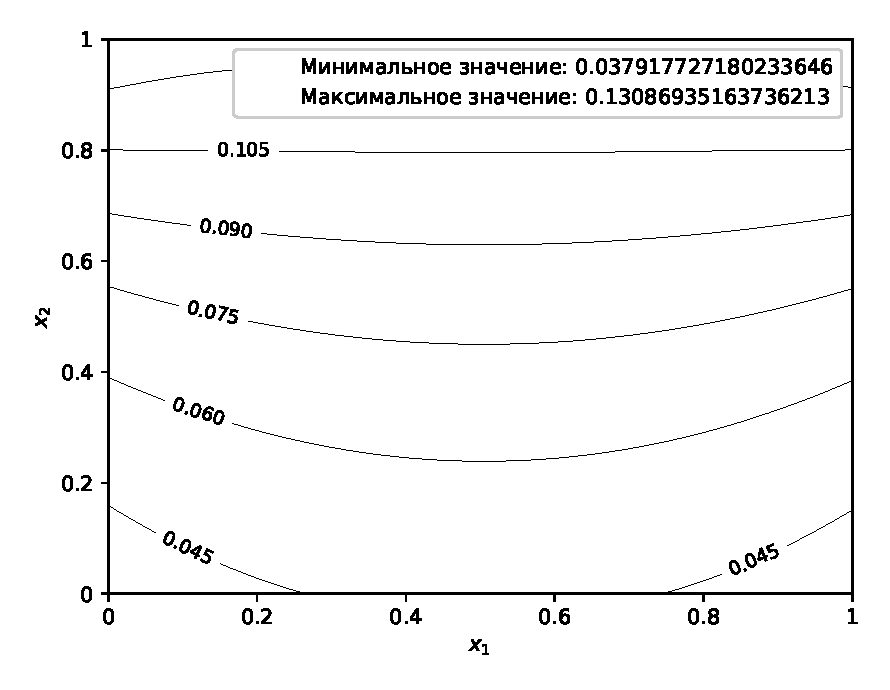
\includegraphics[width=1\linewidth]{boundary/theta_iso_auto} \\ а) $\theta$
        \end{minipage}
        \hfill
        \begin{minipage}[b][][b]{0.49\linewidth}
            \centering
            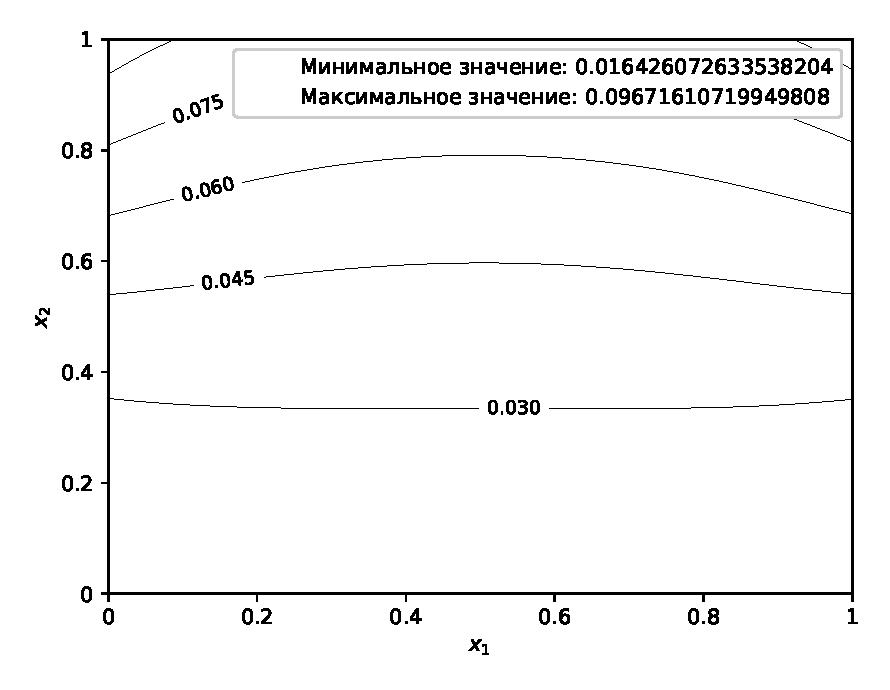
\includegraphics[width=1\linewidth]{boundary/phi_iso_auto} \\ б) $\varphi$
        \end{minipage}
        \caption{Решение граничной задачи в двумерной области}
        \label{fig:4_1:boundary}
    \end{figure}
\end{frame}

\begin{frame}

    \textbf{Пример 2} (трёхмерная область).
    Пусть $\Omega=\{(x,y,z),\, 0 \leq x,y,z \leq 1 \}$.
    Определим функции $\gamma, \theta_b$ следующим образом:
    $\gamma = 0.8 \cos\left(\frac{\pi}{2} z\right) + 0.5$,
    $\theta_b = 1- y / 2 + z /2$.

    Начальное приближение также выберем нулевым.
    Для нахождения состояния потребовалось шесть итераций,
    результат представлен на рисунке~\ref{fig:4_1:boundary_3d}.
    \begin{figure}[h!t]
        \begin{minipage}[b][][b]{0.49\linewidth}
            \centering
            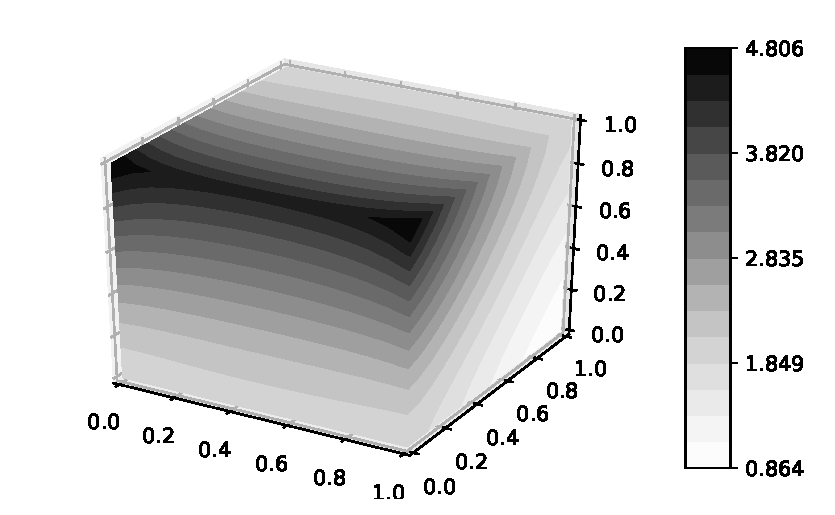
\includegraphics[width=1\linewidth]{boundary/theta_3d} \\ а) $\theta$
        \end{minipage}
        \hfill
        \begin{minipage}[b][][b]{0.49\linewidth}
            \centering
            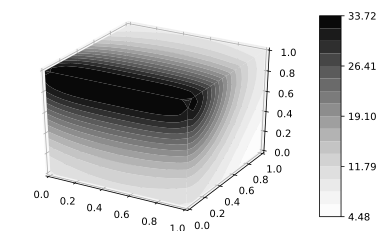
\includegraphics[width=1\linewidth]{boundary/phi_3d} \\ б) $\varphi$
        \end{minipage}
        \caption{Решение граничной задачи в трёхмерной области}
        \label{fig:4_1:boundary_3d}
    \end{figure}
\end{frame}

\subsection{Решение граничных обратных задач}
\begin{frame}
    \frametitle{Нахождение квазирешения обратной задачи}
    \begin{gather}
        A_1 \theta + b \kappa_a (| \theta | \theta^3 - \varphi ) =
        f, A_2 \varphi + \kappa_a (\varphi - |\theta|\theta^3) + F(\varphi, u) = g.
        \label{eq:2_1:weakOperational}\\
        J(\theta) = \frac{1}{2} \int_{\Gamma_2} (\theta - \theta_0)^2 d\Gamma,
        \label{eq:2_1:quality}\\
        A_1 p_1 + 4 |\hat{\theta}|^3 \kappa_a(b p_1 - p_2) = f_c,
        \;\; (f_c,v) = - \int_{\Gamma_2} (\hat{\theta} - \theta_0) v d\Gamma,
        \label{eq:2_1:theorem_2_eq1}\\
        A_2 p_2 + \kappa_a (p_2-b p_1) = g_c(p_2, \hat{u}),
        \;(g_c(p_2, \hat{u}), v) = -\int_{\Gamma_1} \hat{u} p_2 v d\Gamma,
        \label{eq:2_1:theorem_2_eq2}\\
        \int_{\Gamma_1} p_2 (\hat{\varphi} - \theta_b^4)(u-w) d\Gamma
        \leq 0 \quad \forall w \in U_{ad}. \label{eq:2_1:theorem_2_eq3}
    \end{gather}
    \textbf{Алгоритм градиентного спуска с проекцией}
    \begin{enumerate}
        \item Выбор шага $\lambda$, числа итераций $N$, управления $u_0 \in U_{ad}$.
        \item для $k \leftarrow 0,1,2, \ldots, N$ выполнить:
        \begin{itemize}
            \item Для $u_{k}$, вычислить $y_k = \{\theta_k, \varphi_k\}$ из~\eqref{eq:2_1:weakOperational}.
            \item Вычислить значение $J(\theta_k)$ из уравнения~\eqref{eq:2_1:quality}.
            \item Рассчитать $p_k=\{p_{1k},p_{2k}\}$
            из~\eqref{eq:2_1:theorem_2_eq1}--\eqref{eq:2_1:theorem_2_eq2},
            \item Пересчитать управление
            $u_{k+1} = P_{ad}\left[ u_k - \lambda (\varphi_k - \theta_b^4)p_{2k} \right]$.
        \end{itemize}
    \end{enumerate}
\end{frame}

\begin{frame}
    \frametitle{Численное моделирование двумерного случая}
    Положим $\Omega = \{(x,y), 0 \leq x,y \leq 1\}$, $l = 1$ см.
    Граница $\partial\Omega$:
    \[
        \begin{aligned}
            \Gamma_0 & = \{x=\{0,1\}, y \in [0,1]\} \\
            \Gamma_1 & = \{x\in [0,1], y=0\}
            - \text{участок с неизвестными отр. свойствами}, \\
            \Gamma_2 & = \{x \in [0,1], y=1\} - \text{участок наблюдения}.
        \end{aligned}
    \]
    Будем также далее считать, что $a = 0.006[\text{см}^2/\text{c}]$,
    $b=0.025[\text{см}/\text{с}]$, $\beta = 0.00005[\text{см}/\text{с}]$,
    $\kappa=1[\text{см}^{-1}]$, $\kappa_s = 0$, $A = 0$, $\gamma = 0.3$.
    Температуру на границе $\Omega$ положим равной $\theta_b = (x^2+y^2)/3$.

    При указанных параметрах для первого эксперимента выберем следующее тестовое
    значение функции $u$:
    \begin{equation*}
        u(x)=
        \begin{cases}
            0.01, & \text{если } x \le 0.5, \\
            0.5, & \text{если } x > 0.5,
        \end{cases}
    \end{equation*}
    и для второго эксперимента:
    $u(x)=0.49x+0.01$.
\end{frame}


\begin{frame}
    \frametitle{Результаты моделирования обратной граничной задачи}
    \centering
    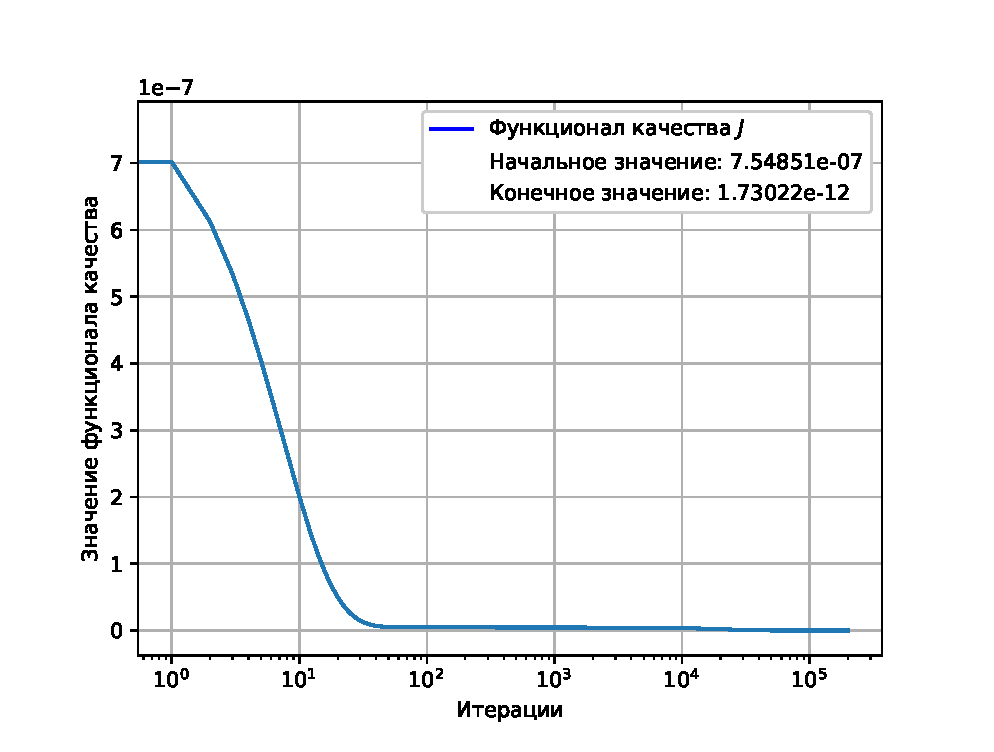
\includegraphics[width=0.495\linewidth]{dvmg368/3}
    \includegraphics[width=0.495\linewidth]{dvmg368/4}
    \includegraphics[width=0.495\linewidth]{dvmg368/1}
    \includegraphics[width=0.495\linewidth]{dvmg368/2}
\end{frame}

\subsection{Решение задачи оптимального управления для квазистационарной модели}\label{quasi-solve}
\begin{frame}
    \frametitle{Моделирование квазистационарного процесса}
    Задача оптимального управления для квазистационарной модели:
    \begin{equation*}
        J_{\lambda}(\theta, u)=\frac{1}{2} \int_{0}^{T}
        \int_{\Gamma}\left(\theta-\theta_{b}\right)^{2} d \Gamma d t+\frac{\lambda}{2}
        \int_{0}^{T} \int_{\Gamma} u^{2} d \Gamma d t \rightarrow \inf
    \end{equation*}
    при ограничениях
    \begin{gather*}
        \begin{split}
            & \frac{\partial \theta}{\partial t} - a \Delta \theta
            + b \kappa_{a} \left(|\theta| \theta^{3}-\varphi\right) = 0,\\
            & - \alpha \Delta \varphi
            + \kappa_{a} \left(\varphi-|\theta| \theta^{3}\right) = 0,
            \quad x \in \Omega, \quad 0 < t < T;
        \end{split}\\
        a \left(\partial_{n} \theta+\theta\right)=r,
        \quad \alpha\left(\partial_{n} \varphi
        + \varphi\right) = u \text { на } \Gamma;\\
        \left.\theta\right|_{t=0} = \theta_{0}.
    \end{gather*}
    Задача аппроксимирует задачу с данными типа Коши для температуры.
\end{frame}

\begin{frame}
    Область $\Omega \times(-L, L)$,
    где $\Omega=$ $\left\{x=\left(x_{1}, x_{2}\right): 0<x_{1,2}<d\right\}$
    и при большом $L$ сводится к двумерной задаче.

    Определим параметры следующим образом:
    $d=1(\text{м})$, $a=0.9210^{-4}(\text{м}^{2} / \text{с})$,
    $b=0.19(\text{м} / \text{с})$, $\alpha=0.0333(\text{м})$,
    $\kappa_{a}=1\left(\text{м}^{-1}\right)$.
    \begin{figure}[h!t]
        \begin{minipage}[b][][b]{0.49\linewidth}
            \centering
            \includegraphics[width=1\linewidth]{paper03/1} \\ а) Поле температуры,
            полученное в статье *
        \end{minipage}
        \hfill
        \begin{minipage}[b][][b]{0.49\linewidth}
            \centering
            \includegraphics[width=1\linewidth]{paper03/2} \\
            б) Поле температуры, полученное предложенным алгоритмом
        \end{minipage}
        \caption{Сравнение полученных температурных полей}
        \label{fig:4_3:1}
    \end{figure}
    \tiny{* A. Y. Chebotarev, A. E. Kovtanyuk и N. D. Botkin. — \textit{«Problem of
    radiation heat exchange with boundary conditions of the Cauchy type»}. —
    Communications in Nonlinear Science and Numerical Simulation 75 (2019),
        с. 262—269.}
\end{frame}

\subsection{Квазилинейная начально-краевая задача, моделирующая ВВЛА}
\begin{frame}
    \frametitle{Квазилинейная модель в контексте ВВЛА}
    Возьмём оптические и термофизические среды из статьи **.
    Параметры $\theta_{b}$ и $\theta_{i n}$ соответствуют
    температуре $37^{\circ} \text{C}$, коэффициент $\gamma$ равен 1.
    Начальное положение кончика оптического волокна $(r, z)=(0,5)$,
    скорость отката составляет $2 \text{~мм} / \text{с}$.

    \begin{figure}[h!t]
        \includegraphics[scale=0.15]{6_cheb/1}
        \caption{Область вычисления}
        \label{fig:4_3:3}
    \end{figure}
    \tiny{** Peter WM van Ruijven и др. — \textit{«Optical-thermal mathematical model for
    endovenous laser ablation of varicose veins»}. -- Lasers in medical science
    29 (2014), с. 431—439}
\end{frame}


\begin{frame}
    \frametitle{Результаты вычисления}
    \begin{minipage}[t]{0.47\linewidth}
        \small{Поведение температуры в точке $(1.5,10)$
            при мощности лазера $10\text{~Вт}$ и следующих длинах волн:
            $810\text{~нм}$ (черный), $1064\text{~нм}$ (красный),
            $1470\text{~нм}$ (зеленый) и $1950\text{~нм}$ (синий).}
        \center{\includegraphics[width=1\linewidth]{6_cheb/2}}
    \end{minipage}
    \hfill
    \begin{minipage}[t]{0.47\linewidth}
        \small{Поведение температуры в точке $(1.5,10)$
            для следующих длин волн и мощностей лазера:
            $810 \text{~нм}, P=10 \text{~Вт}$ (черный);
            $1064 \text{~нм}, P=11 \text{~W}$ (красный);
            $1470 \text{~нм}, P=7,5 \text{~W}$ (зеленый);
            $1950 \text{~нм}, P=6 \text{~W}$ (синий).}
        \center{\includegraphics[width=1\linewidth]{6_cheb/4}}
    \end{minipage}
\end{frame}

\begin{frame}

\end{frame}
